\chapter{Réalisation}

\section*{Introduction}

\section{Flux de travail}
la meilleure façon de décrire le flux de travail dans notre projet est à travers ce diagramme de Gantt \ref{fig:gantt} qui représente les différentes parties du projet, et sa durée, qui a pris environ 7 mois, le diagramme de Gantt montre les tâches terminées et celles en attente, et les principaux acteurs qui sont GHARAFI Hamza, GHARAFI Ayoub et une équipe de 8 résidents bénévoles.
nous tenons à mentionner que l'obtention des ressources nécessaires pour ce type de projet a été très difficile, et il nous a fallu près d'un mois, pour mettre la main sur HPC-MARWAN et colab pro plus.
\section{Réalisation}
\subsection{Application web}
la réalisation de l'application web a été orientée pour être conviviale tout en étant efficace, d'où l'utilisation de multiples fonctionnalités pour simplifier l'utilisation de l'interface pour nos collaborateurs.
Dans cette section, nous allons afficher certaines des fonctionnalités de l'application Web, pour plus de fonctionnalités, visitez l'annexe

\begin{figure}[H]
    \centering
    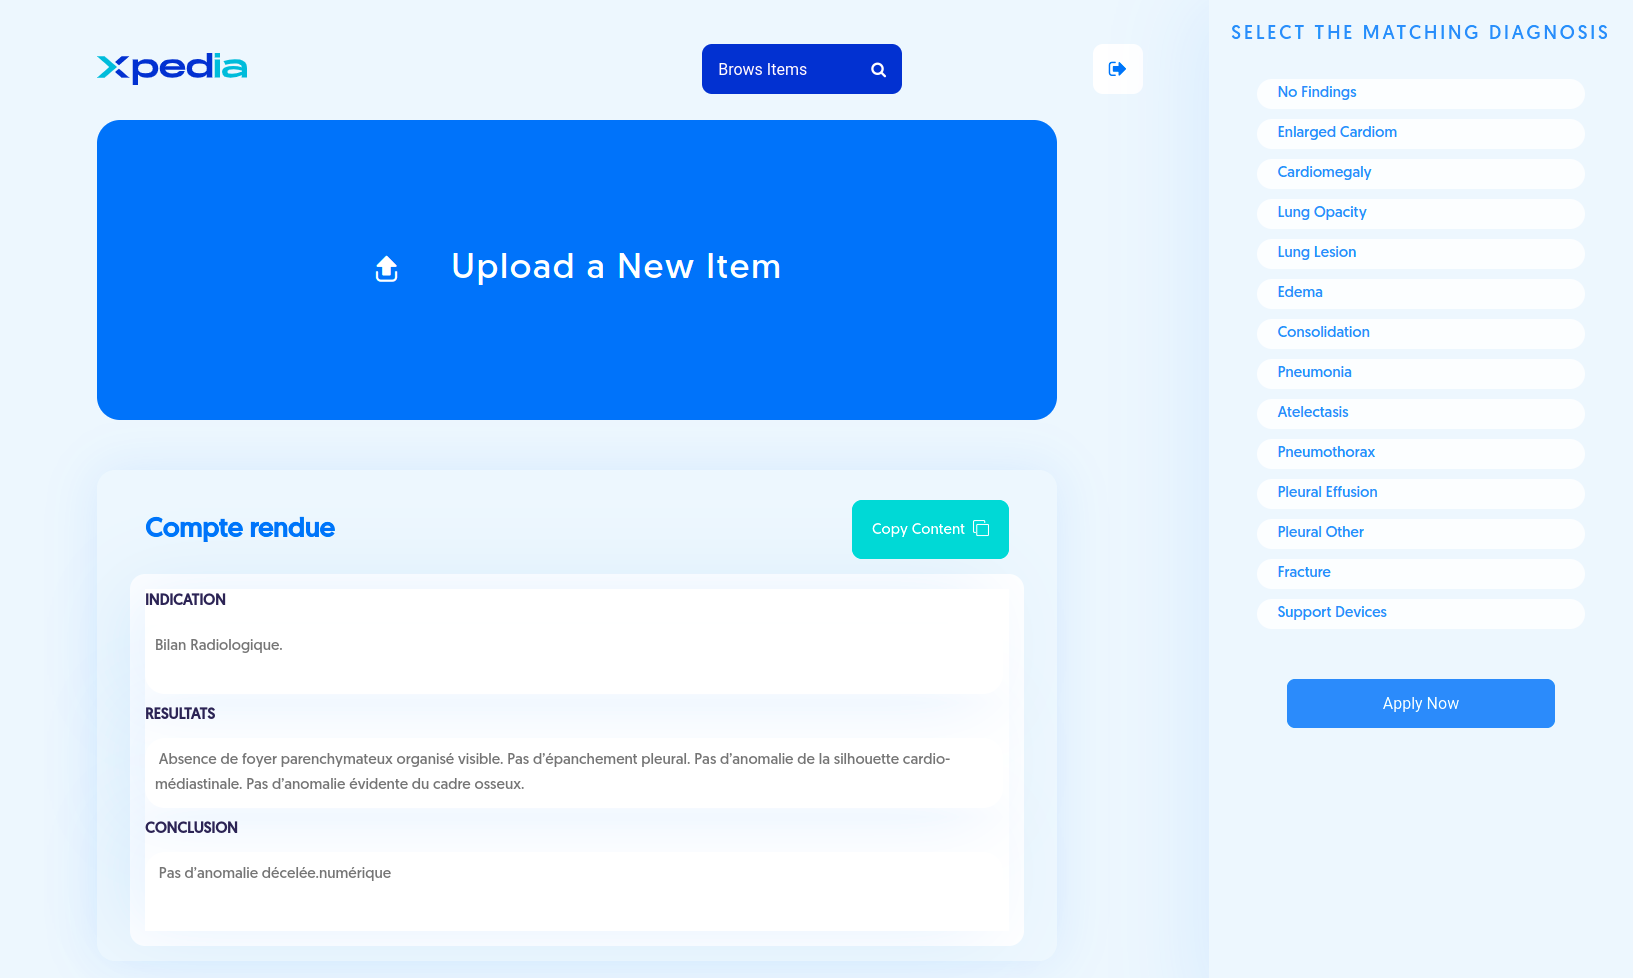
\includegraphics[width=0.8\textwidth]{xpedia_additem.png}
    \caption{La page ajouter élément}\label{fig:xpedia_additem}
\end{figure}
\begin{figure}[H]
    \centering
    
\includegraphics[width=0.8\textwidth]{xpedia_add_image.png}
    \caption{La section réserver à l'ajout d'une image}\label{fig:xpedia_add_image}
\end{figure}
\begin{figure}[H]
    \centering
    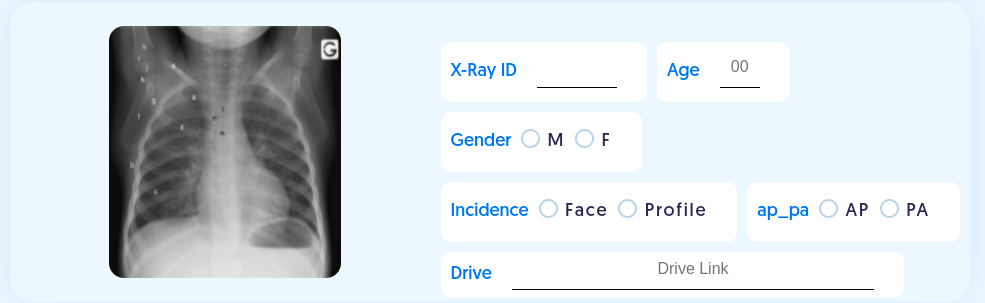
\includegraphics[width=0.8\textwidth]{xpedia_fill_form.png}
    \caption{La formulaire à remplir}\label{fig:xpedia_fill_form}
\end{figure}
\begin{figure}[H]
    \centering
    
\includegraphics[width=0.8\textwidth]{xpedia_normal_select.png}
    \caption{Choix de 'No Finding' diagnostique}\label{fig:nofinding_choice}
\end{figure}
\begin{figure}[H]
    \centering
    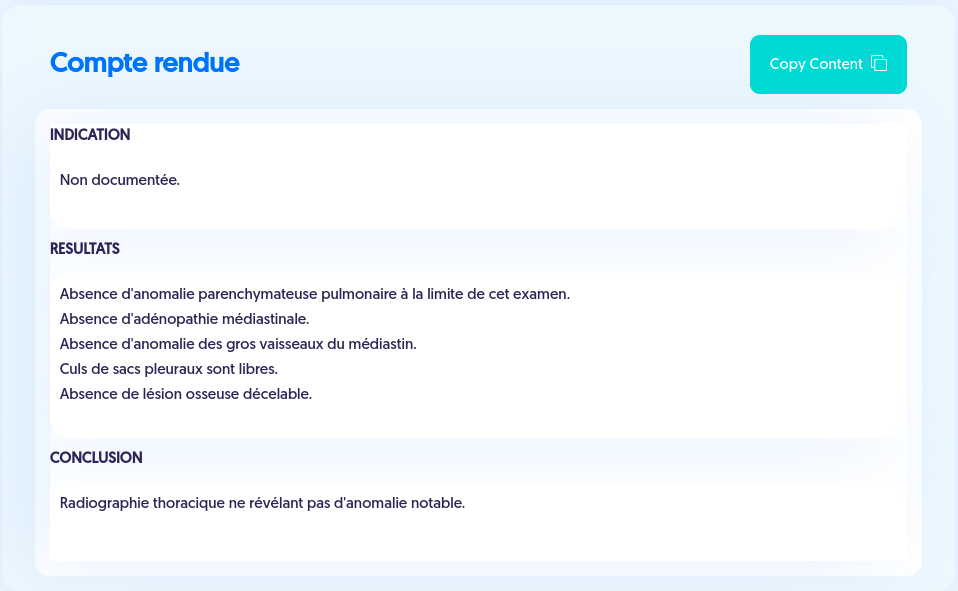
\includegraphics[width=0.8\textwidth]{xpedia_normal_cr.png}
    \caption{Remplissage automatique du compte rendue}\label{fig:xpedia_normal_cr}
\end{figure}
\begin{figure}[H]
    \centering
    
\includegraphics[width=0.8\textwidth]{xpedia_research.png}
    \caption{La bar de recherche}\label{fig:xpedia_research}
\end{figure}

\begin{figure}[H]
    \centering
    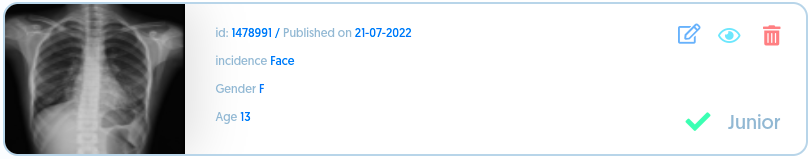
\includegraphics[width=0.8\textwidth]{xpedia_item_thumbnail.png}
    \caption{Vignette de l'élément}\label{fig:xpedia_item_thumbnail}
\end{figure}
\begin{figure}[H]
    \centering
    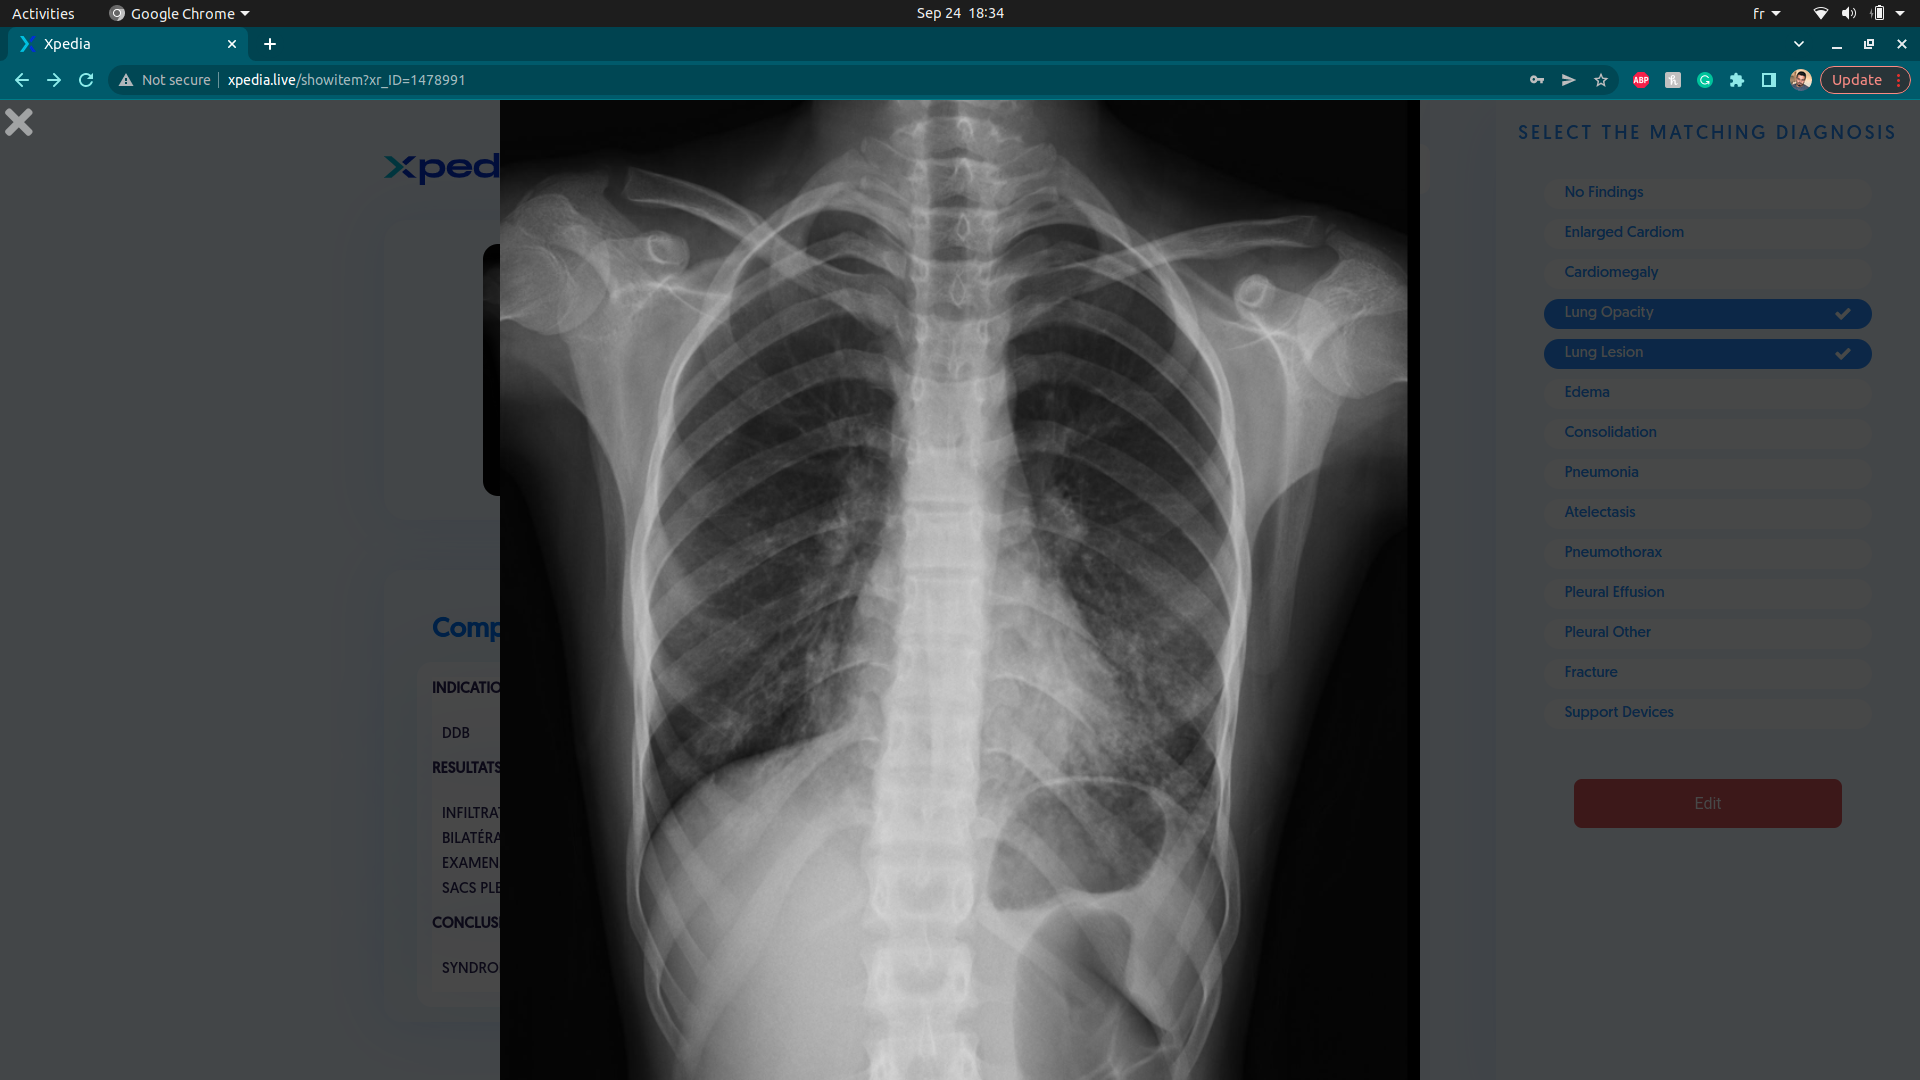
\includegraphics[width=0.8\textwidth]{xpedia_view_showitem.png}
    \caption{Clichés en dimension réel}\label{fig:xpedia_view_showitem}
\end{figure}
\subsection{Preparation des données}
La phase de préparation de données est l'une des phases cruciales dans le projet, le livrable de cette phase est le jeu de données qui alimente le modèle d'apprentissage en profondeur. Pour que ces données soient utiles, elles doivent d'abord être prétraitées selon les étapes déjà décrites dans la section \ref{data_pipeline}. Les figures présentent un exemple de traitement préparatif des données pour l'entraînement, le rest se trouve dans \ref{}.
\begin{figure}[H]
    \centering
    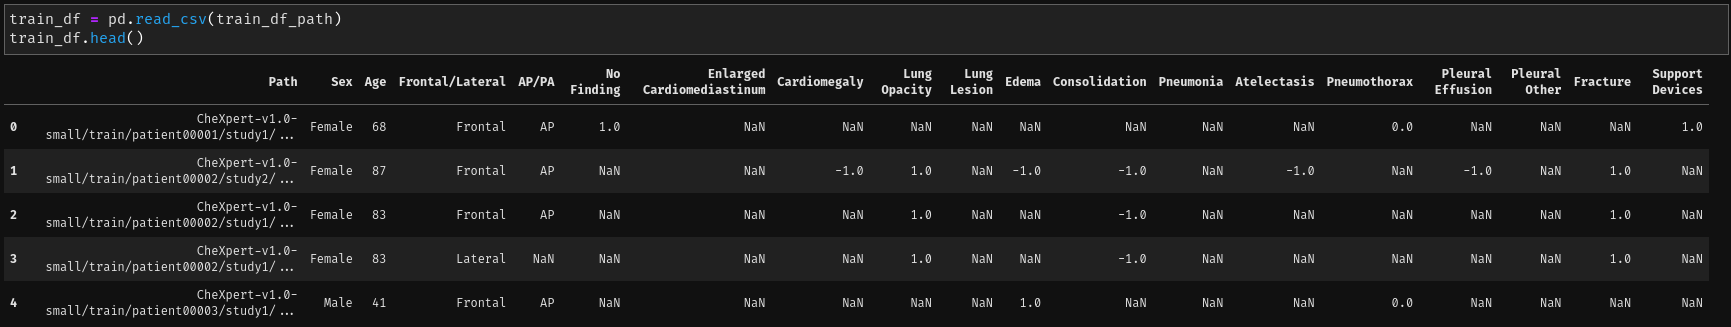
\includegraphics[width=0.8\textwidth]{raw_data.png}
    \caption{Les données brute de la base de données CheXpert}\label{fig:raw_data}
\end{figure}
\begin{figure}[H]
    \centering
    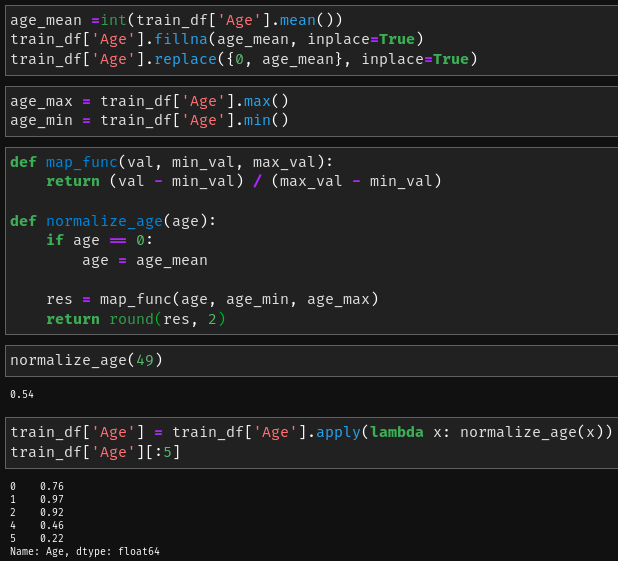
\includegraphics[width=0.8\textwidth]{age_prep.png}
    \caption{La préparation de la colone 'Age'}\label{fig:age_prep}
\end{figure}
\begin{figure}[H]
    \centering
    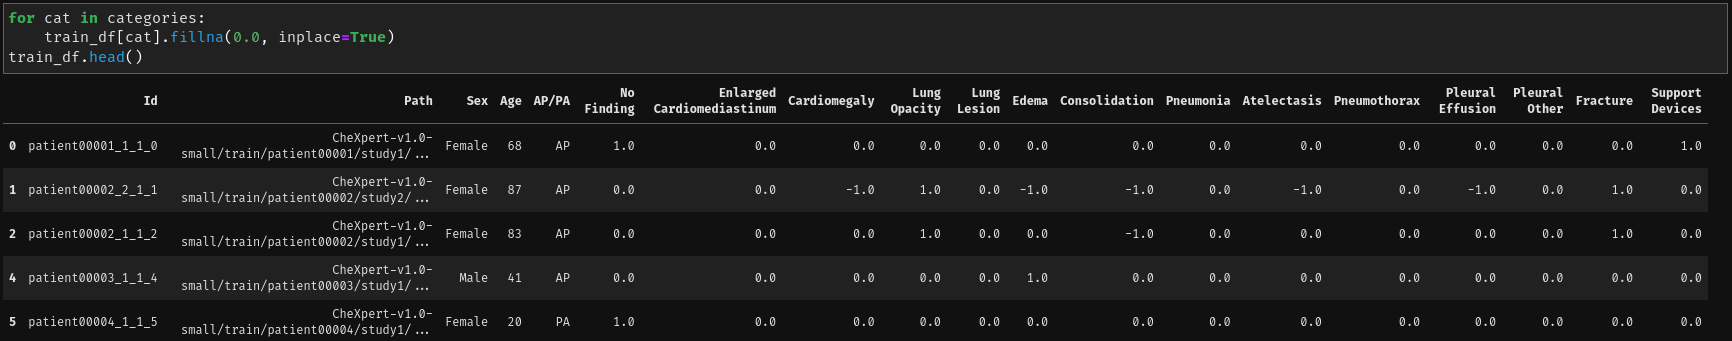
\includegraphics[width=0.8\textwidth]{nan_fill.png}
    \caption{Remplacer les celles vides (Nan)}\label{fig:nan_fill}
\end{figure}

On constate que notre jeu de données comporte plus de 200000 images qui doivent être redimensionnées et convertis en un tableau numpy pour les utiliser comme des entrées dans la phase d'entraînement, cela génère un goulot d’étranglement de flux d’opération. Alors pour anticiper cela on va faire les opérations de prétraitement d’image une seule fois à l'avance et enregistrer le rendu sous forme de fichiers. Et par la suite utiliser ces derniers dans la phase d'entraînement.

\begin{figure}[H]
    \centering
    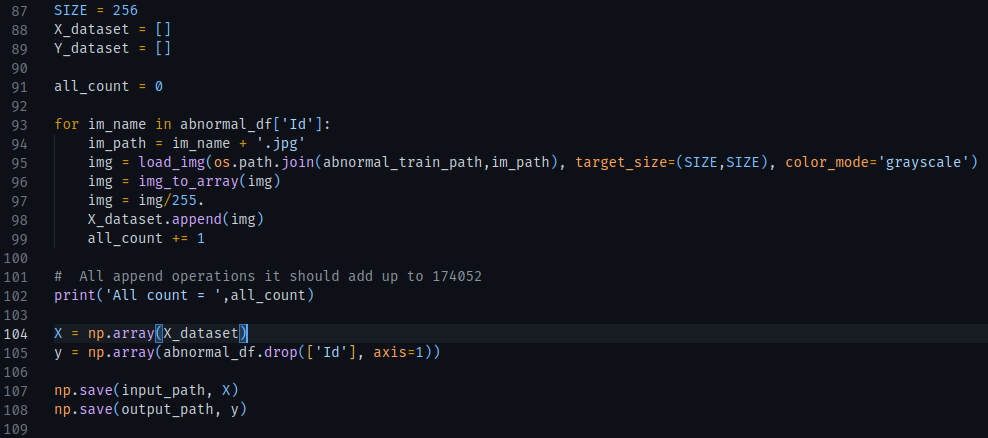
\includegraphics[width=0.8\textwidth]{input_output.png}
    \caption{Préparer les images et meta données pour la phase d'entraînement}\label{fig:input_output}
\end{figure}


\subsection{Madèles d'apprentissage en profondeur}
Dans cette phase, nous avons essentiellement deux voies principales à suivre, comme indiqué sur la figure, la première consiste à créer notre propre modèle et à commencer à l'entraîner sur les données préparées, et la deuxiéme consiste à utiliser un modèle pré-entraîner pour se recycler sur le données préparées, mais quel que soit la voie que nous choisissons, la structure de notre modèle sera la même.
Notre structure n'est pas simple car nous avons deux types de données d'entrée, nous avons donc deux modèles distincts pour traiter chaque type, puis les concaténer dans une couche entièrement connectée pour accéder à notre couche de sortie.
\begin{figure}[H]
    \centering
    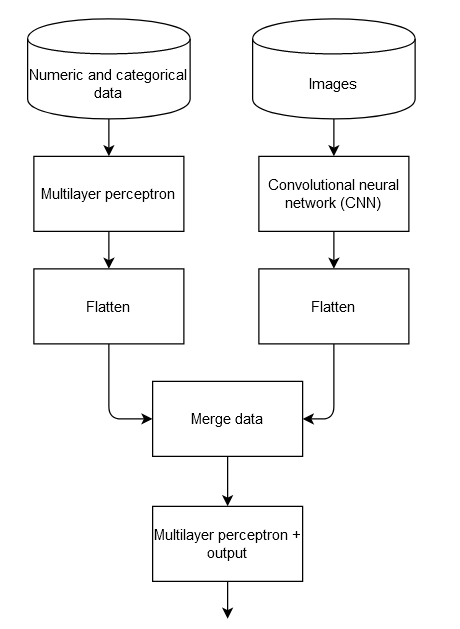
\includegraphics[width=0.8\textwidth]{mixed_inputs.png}
    \caption{L'historique des experiences des modèles de classification binaire}\label{fig:binary_history}
\end{figure}
Dans les paragraphes suivants, nous parlerons des couches et de modèles Keras.
D’abord en commençant par le modèle binaire pour classer les données normales et anormales, pour le modèle de traitement d'images nous allons construire un modèle séquentiel contenant:
\begin{enumerate}
    \item couche Conv2D avec la fonction d'activation Relu
    \item couche de BatchNormalization
    \item Couche de Maxpooling
    \item Couche de Dropout (pas toujours)
\end{enumerate}
En répétant ces 4 couches 3 à 4 fois en réglant les paramétres relatives à chaque couche (nombre de filtres, taille de pooling, valeur de dropout …) on va avoir la partie de base de notre modèle, aprés on va finalisé notre modèle par les couches suivantes:
\begin{enumerate}
    \item couche Flatten
    \item couche Dense avec la fonction d'activation Relu
    \item couche Dropout
    \item couche Dense avec la fonction d'activation Relu
    \item couche Dropout
    \item couche Dense avec la fonction d'activation Sigmoid
\end{enumerate}
\begin{figure}[H]
    \centering
    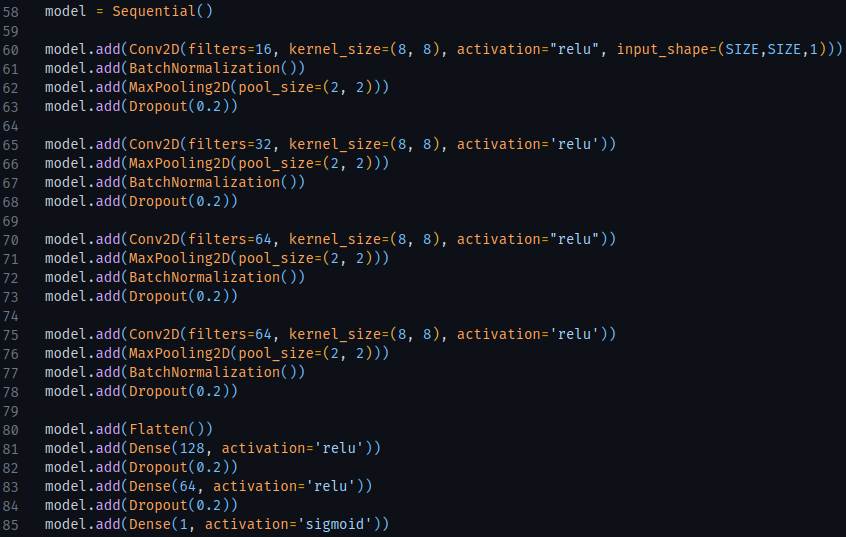
\includegraphics[width=0.8\textwidth]{binary_model_arc.png}
    \caption{L'architecture des RNC}\label{fig:binary_history}
\end{figure}

Puis pour le modèle de traitement du meta données (Age, Sexe, AP/PA), on va utiliser un modèle séquentiel contenant 2 couches Dense avec la fonction d’activation Relu.

Et finalement on doit combiner ces 2 modèle par 2 couches Dense avec fonction d’activation Relu pour avoir la couche de sortie de notre modèle principale.

La sortie de ce modèle et un nombre compris entre 0 et 1.

Pour le modèle multi-etiquettes on aura la même structure avec la différence du format de la sortie qui sera un tableau de valeurs entre 0 et 1, ce dernier représente la probabilité d'existence de chaque pathologie respectivement.


\section{Experiences}

Dans cette partie on aura une vision totale sur les expériences effectuées et les expériences en attente de réalisation en raison du problème de ressources déjà expliqué dans la partie précédente.

Comme on le voit sur la figure \ref{fig:binary_history}, l'historique des expériences faites pour créer un modèle binaire montre qu’après un changement de la taille des images nous avons gardé la même structure tout en incrémentant le nombre d'époques, car il a eu une évolution évidente de la précision du modèle.

\begin{figure}[H]
    \centering
    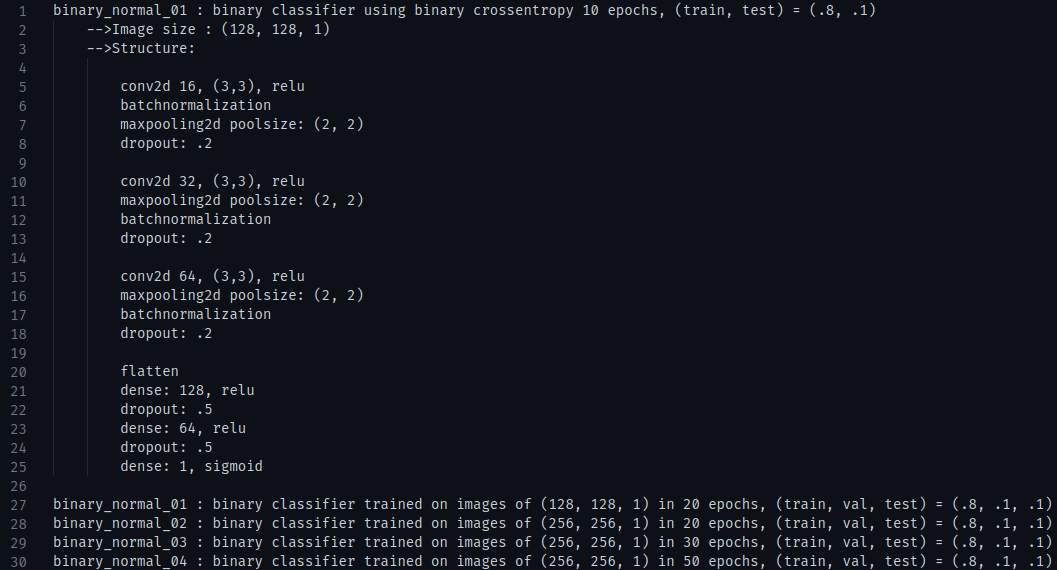
\includegraphics[width=\textwidth]{binary_history.png}
    \caption{L'historique des experiences des modèles de classification binaire}\label{fig:binary_history}
\end{figure}

Pour le modèle multi-étiquettes on a déjà réalisé 6 expériences avec des changements dans les paramètres surtout:
\begin{enumerate}
    \item La taille des filtres pour qu’ils mieux couvre la totalités de l’image sans avoir un débordement
    \item Réduire la taille de Pooling pour ne pas avoir une chute dans la taille du rendu de cette couche
    \item Augmenter la taille des images et finalement varier les valeur de la couche Dropout pour augmenter la valeur du rappel du modèle
    \item Augmenter taille du lot pour avoir un taux d'apprentissage plus grand
\end{enumerate}

\begin{figure}[H]
    \centering
    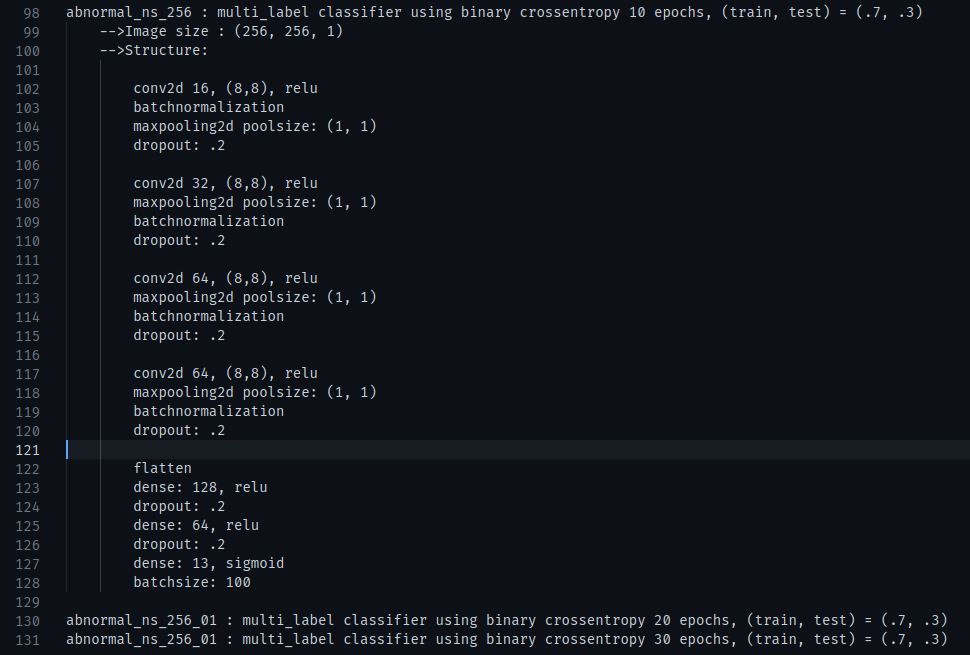
\includegraphics[width=0.8\textwidth]{abnormal_history_01.png}
    \caption{L'historique des experiences des modèles de classification multi-etiquettes 01}\label{fig:abnormal_history_01}
\end{figure}
\begin{figure}[H]
    \centering
    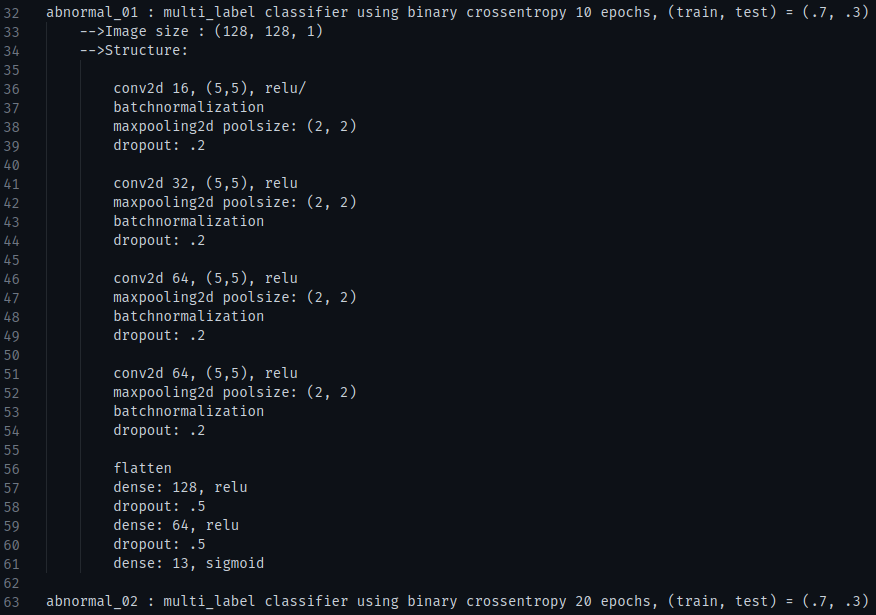
\includegraphics[width=0.8\textwidth]{abnormal_history_02.png}
    \caption{L'historique des experiences des modèles de classification multi-etiquettes 02}\label{fig:abnormal_history_02}
\end{figure}

on n'a pas pu effectuer l'entraînement de toutes les structures créées mais voici quelques exemples d'expériences futures:
\begin{enumerate}
    \item Prends les modèles résultant des expériences précédentes et les alimenter par le jeu de données de la population pédiatrique pour avoir des modèles de classification binaire/multi-etiquettes réservé à la population pédiatrique.
    \item Alimenter un modèle pre-entraîné par les données de la population adulte pour avoir un modèle binaire de classification (normal/anormal).
    \item Alimenter un modèle pre-entraîné par les données de la population adulte pour avoir un modèle de classification multi-etiquettes pour classifier le reste des anomalies.
    \item Réduire le nombre de sortie, en choisissant les anomalies avec la plus grande présence dans la base de données.
    \item Un modèle binaire pour chacune des anomalies, combinées dans un modèle globale par 2 couches Dense une avec La fonction d'activation Relu et la dernière avec la fonction d'activation Sigmoid.
    \item Appliquer l'expérience 1. sur les modèles résultant des expériences 2., 3., 4., 5.
\end{enumerate}

chacune des expériences précédentes aura un certain nombre d'expériences enfants lors du changement des paramètres ou des tailles utilisés.



\section{Résultats}
Cette phase est le fruit de tout le travail effectué sur notre projet jusqu'à présent, Nous commencerons avant tout par les moèles binaires.
    \subsection{Modèle de classification binaire}
        Comme nous l'avons mentionné dans la section expérimentale, nous avons fait quelques expériences, mais en suivant toujours la même structure de modèle, la seule différence est le nombre d'époques. Il suffirait donc de ne montrer que le dernier résultat le plus significatif.
        \begin{figure}[H]
            \centering
            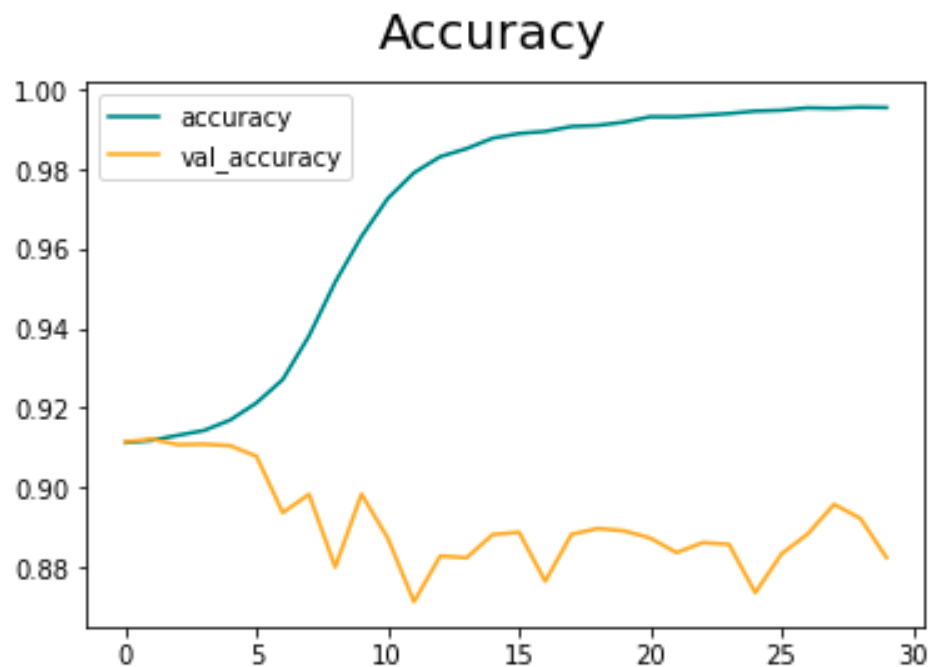
\includegraphics[width=0.5\textwidth]{binary_accuracy.png}
            \caption{La précidion du modèle de classification binaire}\label{fig:binary_accuracy}
        \end{figure}
        \begin{figure}[H]
            \centering
            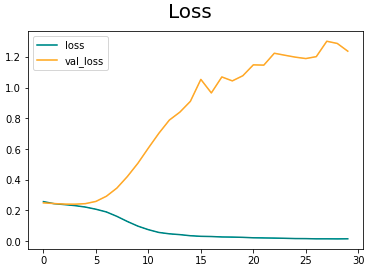
\includegraphics[width=0.5\textwidth]{binary_loss.png}
            \caption{La perte du modèle de classification binaire}\label{fig:binary_loss}
        \end{figure}
        Comme nous le voyons dans les 2 graphiques, se référant à la précision et à la perte de notre modèle binaire, avec une précision d'entraînement de 99,55 et une perte d'entraînement de 0,14, nous pouvons également noter que les valeurs de validation ne sont pas aussi cohérentes que les valeurs d'entraînement, ce qui suggère que notre modèle suradapte les données de formation et se débat avec de nouvelles données de validation ou de test. Une solution pourrait être de simplifier l'architecture du modèle, en réduisant par exemple le nombre de couche, le nombre de nœuds par couche etc.
        Une autre chose qui pourrait contribuer à ce comportement est la différence gigantesque entre le nombre de clichés normaux et anormaux qui rend les données largement déséquilibrées.
        \begin{figure}[H]
            \centering
            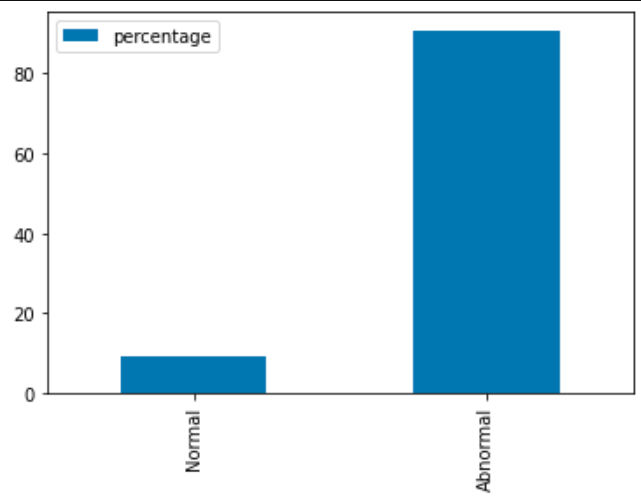
\includegraphics[width=0.5\textwidth]{normal_vs_abnormal.png}
            \caption{La perte du modèle de classification binaire}\label{fig:normal_vs_abnormal}
        \end{figure}
        Après cela et exactement dans la phase de test, nous avons dû utiliser 3 fonctions de test principales, la précision, le rappel et enfin la précision binaire qui en retour nous donne les résultats suivants:
        \begin{enumerate}
            \item La précision: 92.25
            \item Le rappel: 94.99
            \item La précision binaire: 88.19
        \end{enumerate}
        \begin{figure}[H]
            \centering
            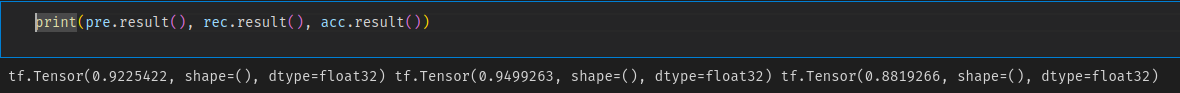
\includegraphics[width=\textwidth]{testing_results.png}
            \caption{Les résultat de la phase de test}\label{fig:testing_results}
        \end{figure}
        Et c'est un exemple d'application de notre modèle, étiqueté par le diagnostic prédit par rapport à celui d'origine.
        Par exemple le premier cas est un cliché normal prédit par le modèle comme étant normal, donc la prédiction est correcte dans ce cas, il en va de même pour les 4 autres clichés qui suivent, par contre le dernier cas est celui d'un cliché normal prédit comme étant anormal, ce qui n'est pas le cas.
        \begin{figure}[H]
            \centering
            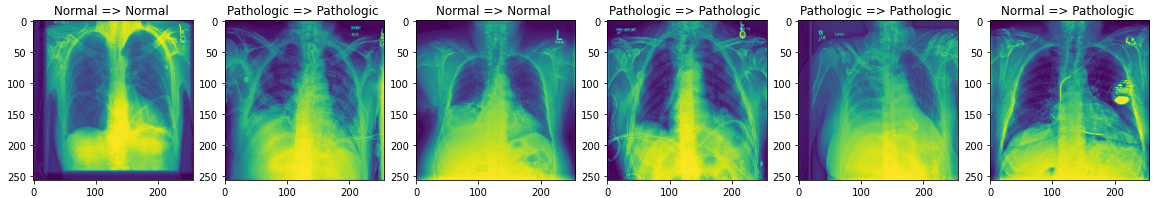
\includegraphics[width=\textwidth]{example_app.png}
            \caption{Exemple d'application du modèle de classification binaire}\label{fig:example_app}
        \end{figure}
    \subsection{Modèle de classififcation multi étiquettes}
        En ce qui concerne nos modèles multi-étiquettes, comme nous l'avons dit dans la section des expériences, nous avons eu quelques expériences sans bons résultats, nous pouvons certainement voir que la précision de la formation augmente dans certaines diagrames \ref{fig:multi_accuracy}, mais c'est une incrémentation minuscule.
        \begin{figure}[H]
            \centering
            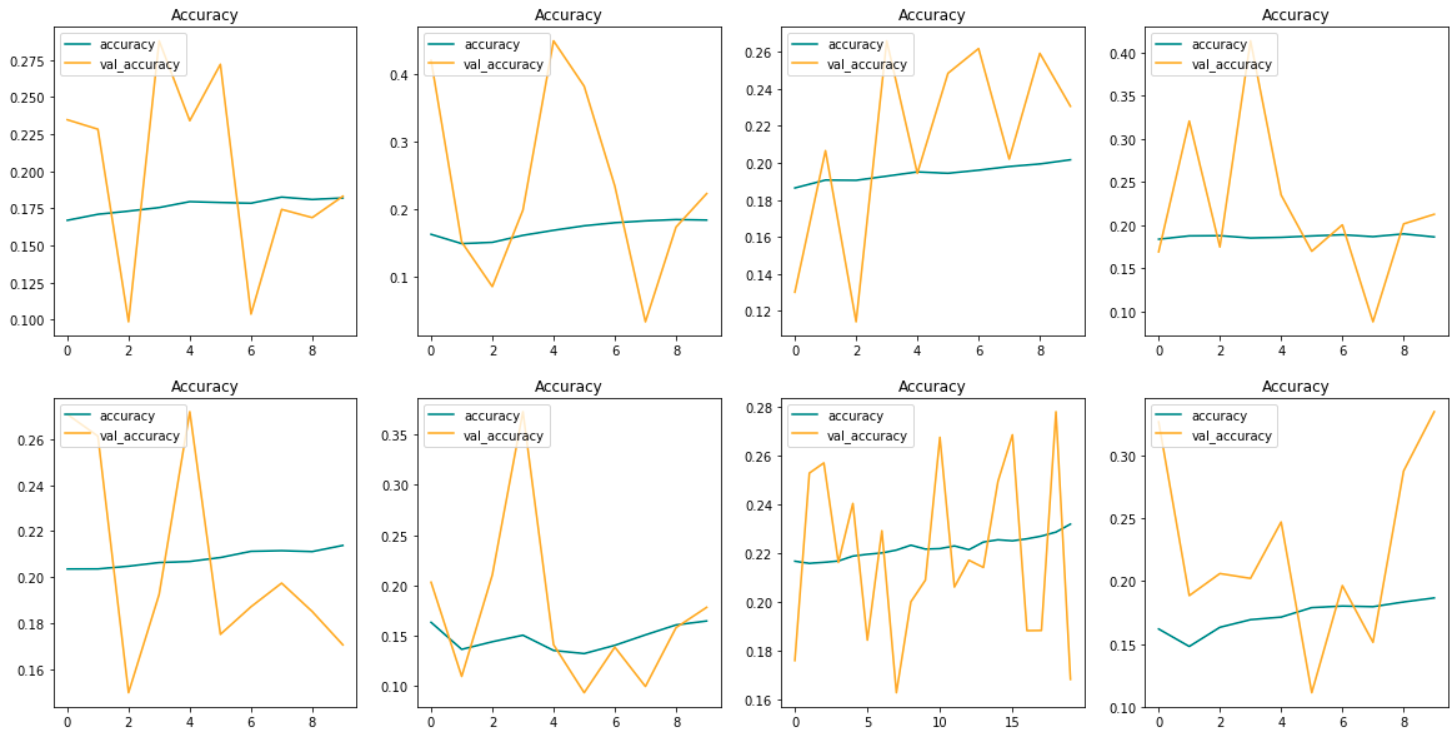
\includegraphics[width=\textwidth]{multi_accuracy.png}
            \caption{La perte du modèle de classification multi étiquettes}\label{fig:multi_accuracy}
        \end{figure}
        La même chose peut être remarquée dans les diagrammes de perte \ref{fig:multi_loss}, nous devons donc soit augmenter de manière exponentielle le nombre d'époques, ce qui est un cauchemar de temps et de consommation informatique, sachant qu'une seule époque peut prendre plus de 2 heures avec un cluster de 8 processeurs, soit nous devons changer notre stratégie et/ou structure de modèle, mais attendez, si nous examinons attentivement ce que le modèle essaie d'accomplir
        \begin{figure}[H]
            \centering
            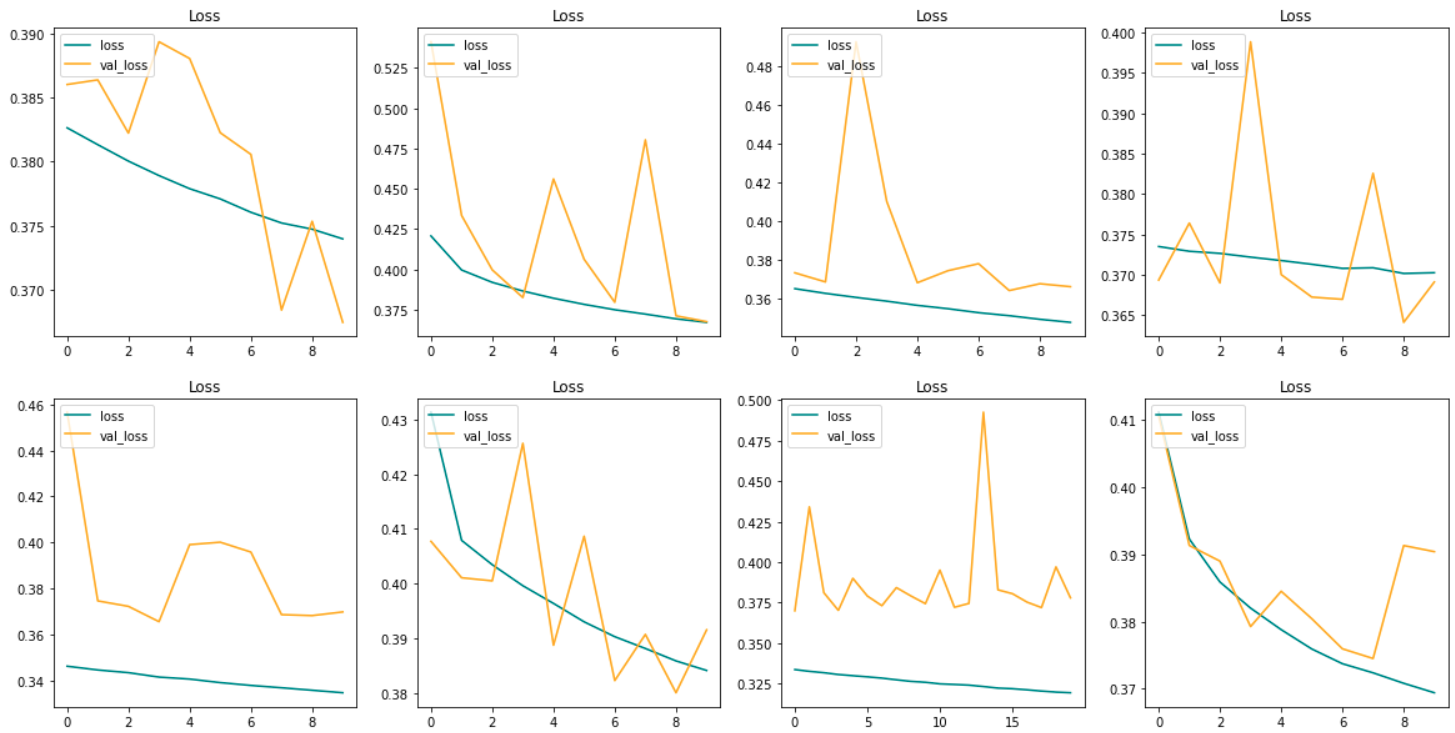
\includegraphics[width=\textwidth]{multi_loss.png}
            \caption{La perte du modèle de classification multi étiquettes}\label{fig:multi_loss}
        \end{figure}
        Nous remarquerons qu'il essaie de comparer un tableau binaire avec un tableau de valeurs continues, en calculant la perte à l'aide de la fonction <binary cross entropy>, donc si une seule des 13 cellules est éteinte, c'est considéré comme une perte, d'où la faible précision de notre modèle, un problème dû à la grande dimensionnalité de nos étiquettes, ce qui nous incite à revivre nos expérimentations non faites, notamment la réduction de dimension et les modèles binaires pour chaque étiquette.
        
\section*{Conclusion}
jusqu'à ce point du projet, nous n'avons fait que franchir quelques étapes et il y en a d'autres à venir surtout les expériences en attente, pour qu'on puisse améliorer la précision des modèles multi étiquettes et en même temps restructurer le modéle de classification binaire pour éviter la suradaptation.

